\documentclass{report}
\usepackage[margin=1in]{geometry} 
\usepackage{amsmath,amsthm,amssymb,amsfonts}
\usepackage{tabto}
\usepackage[yyyymmdd]{datetime}
\renewcommand{\dateseparator}{--}
\newcommand{\N}{\mathbb{N}}
\newcommand{\Z}{\mathbb{Z}}

% For definitions
%\newtheorem{defn}{Definition}[section]
%\newtheorem{thrm}{Theorem}[section]
%\newtheorem{ex}[Example}[section]
\newtheorem*{ex}{Example}
\newtheorem*{defn}{Definition}
\newtheorem*{thrm}{Theorem}
\newtheorem*{lemma}{Lemma}
\newtheorem*{result}{Result}


% For circled text
\usepackage{tikz}
\newcommand*\circled[1]{\tikz[baseline=(char.base)]{
            \node[shape=circle,draw,inner sep=0.8pt] (char) {#1};}}

\usepackage{pgf}
\usetikzlibrary{arrows, automata}

% For equation system alignment
\usepackage{systeme,mathtools}
% Usage:
%	\[
%	\sysdelim.\}\systeme{
%	3z +y = 10,
%	x + y +  z = 6,
%	3y - z = 13}

\newenvironment{problem}[2][Problem]{\begin{trivlist}
\item[\hskip \labelsep {\bfseries #1}\hskip \labelsep {\bfseries #2.}]}{\end{trivlist}}
%If you want to title your bold things something different just make another thing exactly like this but replace "problem" with the name of the thing you want, like theorem or lemma or whatever
 
%used for matrix vertical line
\makeatletter
\renewcommand*\env@matrix[1][*\c@MaxMatrixCols c]{%
  \hskip -\arraycolsep
  \let\@ifnextchar\new@ifnextchar
  \array{#1}}
\makeatother 
 
% Change chapter numbering
\newcommand{\mychapter}[2]{
	\setcounter{chapter}{#1}
	\setcounter{section}{0}
	\chapter*{#2}
	\addcontentsline{toc}{chapter}{#2}
}

\usepackage{graphicx}
\graphicspath{ {images/} }

\begin{document}
 
\tableofcontents{}
\mychapter{1}{2018-01-30}
\section{Depth First Search (DFS)}
\begin{defn}
For graph $G$:\\
You start with $S$ and try first edge leading to $V$. Then you follow the first edge leading out of $V$. Continue like this until you reach a dead end. Then backtrack until you get to node with an unvisited node.
\end{defn}
\subsection{BFS vs DFS}
Similarities:
	\begin{itemize}
	\item Cross through all the nodes.
	\item Similar level of efficiency.
	\end{itemize}
Differences:
	\begin{itemize}
	\item Ordering of nodes are very different.
	\end{itemize}

\subsection{DFS (u)}
	\begin{verbatim}
	Mark u as explored and add u to R
	Foreach edge (u,v) incident to v
	  IF v is not marked as explored then
	    recursively invoke DFS(v)
	  Endif
	Endfor
	\end{verbatim}

\subsection{Adjacency Matrix/ Adjacency List}
Matrices are nice for understanding graphs but they aren't nice for implementing them since they use space $O(n^2)$.\\
\begin{ex}
Given we have $n$ vertices and $m$ edges:\\
Adjacency matrix has space complexity of $O(n+m)$ when given a sparse graph meaning the number of edges is not much larger than the number of nodes. Since there are $n+m$ representations of the graph, then going through the structure (identifying all edges) will also take $O(n+m)$ time.
\end{ex}
\begin{ex}
Given a matrix with N=100 items and a cost of $c$. Then the max cost is $100c$.\\
Then the number of elements in the list will be 100 and the time to traverse the list will be $100c$ in other words $(n+m)c$ where $(n+m)$ is the entire representation of the graph.
\end{ex}

Adjacency List needs $O(n+m)$ space for sparse graphs.
\begin{enumerate}
\item Array Adj where Adj[v] is a record containing the list of all nodes adjacent to $v$.
\item For undirected graph $G(V,E)$ each edge $e(v,w)$ occurs on two adjacency lists: node w appears on the list for node $v$, node $v$ appears on the list for node $w$.
\item Need an array of pointers of length n to setup list in Adj; we need the space for all the lists.
\item Length of the list may vary but in (1) and (2) $e(v,w)$ appears in exactly two of the lists: One for $v$ and one for $w$. Thus the total length of all the lists is $2m$. \qed
\end{enumerate}
Best case space complexity for list is $\Omega(n)$, worst case is $O(n^2)$ for when graph is complete, and average case is $\Theta(m+n)$.\\
BFS Traversal is $O(n+m) = O(n^2)$.

\mychapter{2}{2018-02-06}
\section{Topological Sorting}
\subsection{Sorting Directed Acyclic Graph}
\begin{thrm}
If $G$ has a topological ordering then $G$ is a DAG (Directed Acyclic Graph).\\
The converse is also true. So if $G$ is a DAG, then $G$ has a topological order.
\end{thrm}
\begin{ex}
Below is a directed acyclic graph $G$ and its topological sorting.
\begin{center}
\includegraphics[scale=0.5]{TopSortingGraph1.png}\\
\includegraphics[scale=0.5]{TopologicalSorting1.png}
\end{center}
\end{ex}
Testing graph functions in \LaTeX
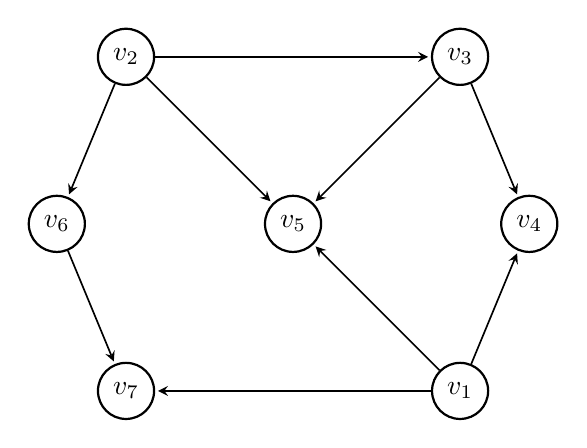
\begin{tikzpicture}[> = stealth,shorten > = 1pt,auto,node distance = 3cm,semithick]
\tikzstyle{every state}=[draw = black,thick,fill = white,minimum size = 4mm]
	
	\node[state] (v5) {$v_5$};
	\node[state] (v7) [below left of=v5] {$v_7$};
	\node[state] (v4) [right of=v5] {$v_4$};
	\node[state] (v6) [left of=v5] {$v_6$};
	\node[state] (v2) [above left of=v5] {$v_2$};
	\node[state] (v3) [above right of=v5] {$v_3$};
	\node[state] (v1) [below right of=v5] {$v_1$};
	
	\path[->] (v1) edge node {} (v4);
	\path[->] (v1) edge node {} (v7);
	\path[->] (v1) edge node {} (v5);
	\path[->] (v2) edge node {} (v6);
	\path[->] (v2) edge node {} (v5);
	\path[->] (v2) edge node {} (v3);
	\path[->] (v3) edge node {} (v5);
	\path[->] (v3) edge node {} (v4);
	\path[->] (v6) edge node {} (v7);
\end{tikzpicture}

\subsection{Divide and Conquer}
Divide and Conquer is a strategy of solving problems by splitting a task into smaller pieces and working on each piece individually.\\
This system also allows us to merge the pieces back together in linear time.\\
\subsection{Insertion Sort}
Step or moment of key:\\
$\Theta(N)$ steps in terms of key positions = $\Theta(N)$ time.
$\Theta(N^2)$ time.\\
Can we make this algorithm better than $\Theta(N^2)$?





\end{document}